\documentclass[tikz,border=2mm]{standalone}
\usetikzlibrary{shapes.geometric, arrows}

\tikzstyle{box} = [rectangle, draw=gray, thick, text centered, rounded corners, minimum height=1cm, minimum width=2.5cm, fill=gray!10]
\tikzstyle{arrow} = [thick,->,>=stealth]
\tikzstyle{doublearrow} = [thick,<->,>=stealth]
\tikzstyle{note} = [red, text width=4cm, font=\small\it]

\begin{document}

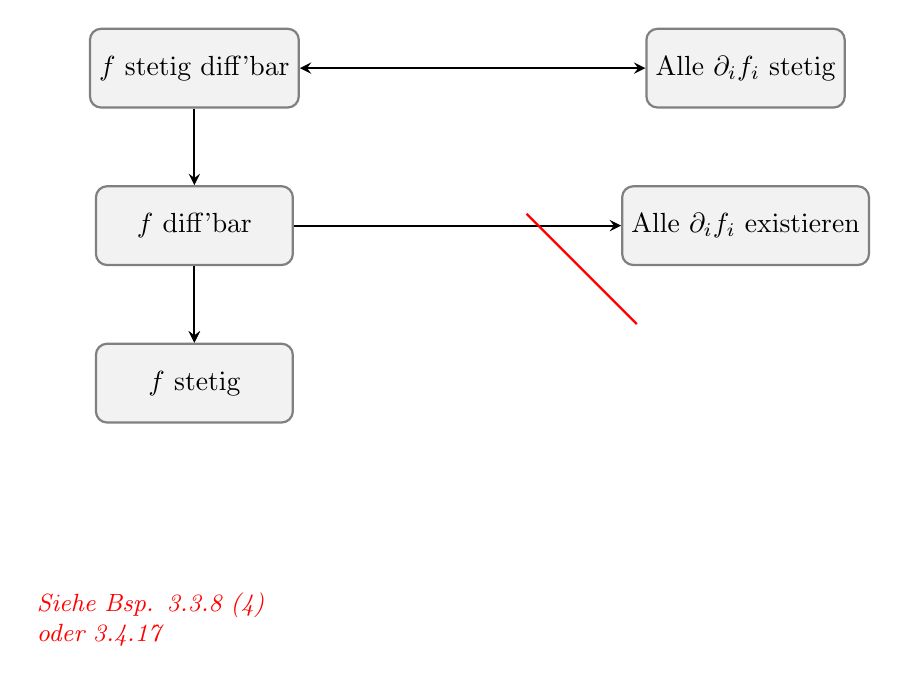
\begin{tikzpicture}[node distance=2cm]

    % Nodes
    \node (f_stetig_diffbar) [box] {$f$ stetig diff'bar};
    \node (parti_stetig) [box, right of=f_stetig_diffbar, xshift=5cm] {Alle $\partial_i f_i$ stetig};
    \node (f_diffbar) [box, below of=f_stetig_diffbar] {$f$ diff'bar};
    \node (parti_existieren) [box, right of=f_diffbar, xshift=5cm] {Alle $\partial_i f_i$ existieren};
    \node (f_stetig) [box, below of=f_diffbar] {$f$ stetig};

    % Arrows
    \draw [doublearrow] (f_stetig_diffbar) -- (parti_stetig);
    \draw [arrow] (f_diffbar) -- (parti_existieren);
    \draw [arrow] (f_diffbar) -- (f_stetig);
    \draw [arrow] (f_stetig_diffbar) -- (f_diffbar);
    \draw [arrow] (f_diffbar) -- (f_stetig);

    % Crossed-out arrow
    \draw[thick, red] (parti_existieren.west) ++(-1.2cm, 0.15cm) -- ++(1.4cm, -1.4cm);

    % Notes
    \node [note, below of=f_stetig, yshift=-1cm] {Siehe Bsp. 3.3.8 (4) \\ oder 3.4.17};

\end{tikzpicture}

\end{document}
